\scanpage{219}\mspage{164}

% MS 1–4
Sous forme duale d'un th. de chgt. de base pour $f_*^{\mathbb D}$, par chgt de base $\mathbb D$-lisse, c'est fait dans I p.~\unsure{56|66} ; 58, et on doit pouvoir l'appliquer ici.

% MS 4–11
\deleted{Nous} Notons que dans la dém. du th. \unsure{loc. cit.}, on n'utilise que l'existence des $f_*^{\mathbb D}$ \inserted{\unsure{L 4 i.e.|L 4 inv.}}, à l'exclusion des $f_!^{\mathbb D}$ \inserted{(L $4'$)}, plus L 5 bien sûr, donc la forme duale ne \deleted{\unsure{doit pas}} fait \unsure{appel} à l'existence des $f_*^{\mathbb D}$, seulement des $f_!^{\mathbb D}$, On a donc une bonne chance de pouvoir l'appliquer à $\mathrm{HOT}_{\unsure{W|w}}$ (où je n'ai pas encore établi l'existence des $f_*^{\mathrm{HOT}}$).

% MS 12
Notons d'abord

% MS left edge of proposition
\margin{\figure{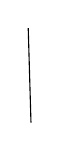
\begin{tikzpicture}[x=1mm,y=1mm]\draw (0,0)--(-0.35,12);\end{tikzpicture}}}

% MS 13–17
\uline{Proposition} 5. Soit $f:S'\longrightarrow S$ une flèche dans $\mathrm{Cat}$. Alors $f$ est une $\mathrm{HOT}_W$-équivalence \uuline{sss} \deleted{c'est une \unsure{Hot} $f$ est dans $W$.} \inserted{$\mathrm{hot}_W(f)$ est iso.} Si $W$ est fortement saturé, cela signifie donc que \deleted{\unsure{ssi}} $f\in W$ (et \unsure{$=$} \unsure{en fait contenu} \inserted{$f\in W\Rightarrow$ une $\mathrm{HOT}_W$-équivalence} dans le \unsure{$+$} démonstration de Der 3 b \deleted{\unsure{tantôt}}.

% MS left beside proposition
% slanted
\margin{devrait remonter avec le th.~3 p.~159}

% MS 17–19
Je rappelle que $f$ est une $\mathrm{HOT}$-équiv., par définition, sss pour \deleted{\unsure{les couples}} $a,b\in\mathrm{Hot}_W$ ($=\mathrm{HOT}_W(e)$),

% MS 20
\[
 \mathrm{Hom}_{\mathrm{HOT}_W(S)}(a_S,b_S)\unsure{\mathord{-}|\longrightarrow}
 \mathrm{Hom}_{\mathrm{HOT}_W(S')}(a_{S'},b_{S'})
\]

% MS 21–24
est iso, où $a_S$ \unsure{etc|est} désigne $p_S^*(a)$ etc ($p_S:S\longrightarrow e$). La formule d'adjonction de $p_{S!},p_S^*$ et de $p_{S'!},p_{S'}^*$ permettent d'interpréter la flèche \unsure{ci$_S$|can.} comme

% MS 25
\[
 \mathrm{Hom}_{\mathrm{Hot}_W}\unsure{\in}(p_{S!}(a_S),b)\longrightarrow
 \mathrm{Hom}_{\mathrm{Hot}_W}(p_{S'!}(a_{S'}),b),
\]

% archive sheet number: 218
